\documentclass[12pt, letterpaper]{article}

% -------------------------------------------------------
% Core layout
% -------------------------------------------------------
\usepackage[
  top=1in, bottom=1in,
  left=1.25in, right=1.25in
]{geometry}

% -------------------------------------------------------
% Fonts and typography
% -------------------------------------------------------
\usepackage{newtxtext, newtxmath}   % Times-like serif font (text + math)
\usepackage{microtype}               % Microtypographic improvements
\usepackage[T1]{fontenc}
\usepackage[utf8]{inputenc}

% -------------------------------------------------------
% Line spacing (double-spaced for review submission)
% -------------------------------------------------------
\usepackage{setspace}
\doublespacing

% -------------------------------------------------------
% Mathematics
% -------------------------------------------------------
\usepackage{amsmath, amssymb, amsfonts}

% -------------------------------------------------------
% Tables
% -------------------------------------------------------
\usepackage{booktabs}         % Professional horizontal rules
\usepackage{array}
\usepackage{tabularx}
\usepackage{multirow}

% -------------------------------------------------------
% Figures and captions
% -------------------------------------------------------
\usepackage{graphicx}
\usepackage{float}            % [H] specifier
\usepackage{placeins}         % \FloatBarrier
\usepackage{caption}
\usepackage{subcaption}

\captionsetup{
  font=small,
  labelfont=bf,
  format=plain,
  justification=justified,
  singlelinecheck=false,
  skip=6pt
}

% -------------------------------------------------------
% TikZ
% -------------------------------------------------------
\usepackage{tikz}
\usetikzlibrary{arrows.meta, positioning, shapes.geometric}

% -------------------------------------------------------
% Code listings
% -------------------------------------------------------
\usepackage{listings}
\usepackage{xcolor}

\definecolor{codebg}{HTML}{F8F8F8}
\definecolor{codeframe}{HTML}{CCCCCC}
\definecolor{codekw}{HTML}{0033B3}
\definecolor{codecomment}{HTML}{8C8C8C}
\definecolor{codestring}{HTML}{067D17}

\lstdefinestyle{pystyle}{
  language        = Python,
  backgroundcolor = \color{codebg},
  basicstyle      = \ttfamily\footnotesize\linespread{1.0}\selectfont,
  keywordstyle    = \color{codekw}\bfseries,
  commentstyle    = \color{codecomment}\itshape,
  stringstyle     = \color{codestring},
  numberstyle     = \tiny\color{gray},
  breaklines      = true,
  breakatwhitespace = true,
  frame           = single,
  rulecolor       = \color{codeframe},
  numbers         = left,
  numbersep       = 8pt,
  xleftmargin     = 2em,
  framexleftmargin= 1.8em,
  tabsize         = 4,
  showspaces      = false,
  showstringspaces= false,
  captionpos      = b,
  aboveskip       = 10pt,
  belowskip       = 6pt
}

\renewcommand{\lstlistingname}{Listing}

% -------------------------------------------------------
% Headers and footers
% -------------------------------------------------------
\usepackage{fancyhdr}
\pagestyle{fancy}
\fancyhf{}
\renewcommand{\headrulewidth}{0.4pt}
\fancyhead[L]{\small\textit{Trojan Detection in Deep Neural Networks}}
\fancyhead[R]{\small\textit{Midterm Report}}
\fancyfoot[C]{\thepage}

% -------------------------------------------------------
% Section heading styles
% -------------------------------------------------------
\usepackage{titlesec}
\titleformat{\section}
  {\normalfont\large\bfseries}{\thesection}{1em}{}
\titleformat{\subsection}
  {\normalfont\normalsize\bfseries}{\thesubsection}{1em}{}
\titleformat{\subsubsection}
  {\normalfont\normalsize\bfseries\itshape}{\thesubsubsection}{1em}{}

\titlespacing*{\section}      {0pt}{2.0ex plus .5ex}{1.0ex plus .2ex}
\titlespacing*{\subsection}   {0pt}{1.5ex plus .4ex}{0.8ex plus .1ex}
\titlespacing*{\subsubsection}{0pt}{1.2ex plus .3ex}{0.6ex plus .1ex}

% -------------------------------------------------------
% Lists
% -------------------------------------------------------
\usepackage{enumitem}
\setlist{itemsep=0.25em, topsep=0.5em, parsep=0pt}

% -------------------------------------------------------
% Paragraph spacing (no indent; use inter-paragraph space)
% -------------------------------------------------------
\setlength{\parindent}{1.5em}
\setlength{\parskip}{0pt}

% -------------------------------------------------------
% Hyphenation
% -------------------------------------------------------
\hyphenpenalty=8000
\exhyphenpenalty=8000

% -------------------------------------------------------
% Column types for tables
% -------------------------------------------------------
\newcolumntype{L}[1]{>{\raggedright\arraybackslash}p{#1}}
\newcolumntype{C}[1]{>{\centering\arraybackslash}p{#1}}
\newcolumntype{R}[1]{>{\raggedleft\arraybackslash}p{#1}}

% -------------------------------------------------------
% Hyperlinks (load last)
% -------------------------------------------------------
\usepackage[hidelinks, breaklinks=true]{hyperref}
\graphicspath{{figures/}}

% Global table row spacing
\renewcommand{\arraystretch}{1.35}

% -------------------------------------------------------
% Table of contents style
% -------------------------------------------------------
\renewcommand{\contentsname}{Table of Contents}

% -------------------------------------------------------
\begin{document}

% ============================================================
%  TITLE PAGE
% ============================================================
\begin{titlepage}
  \thispagestyle{empty}
  \centering
  \vspace*{2.5cm}

  {\LARGE\bfseries A Unified Framework for Trojan Detection\\[0.3em]
  and Mitigation in Deep Neural Networks\par}

  \vspace{0.5em}
  {\large\bfseries Midterm Report\par}

  \vspace{2.5cm}

  {\large
    \textbf{Sai Tarrun Pitta}\\[0.3em]
    \textit{CPSC 589 -- Seminar in Computer Science}\\[0.3em]
    Instructor: \textbf{Kenneth Kung}
  }

  \vfill
  {\normalsize \today}
\end{titlepage}

% ============================================================
%  FRONT MATTER
% ============================================================
\pagenumbering{roman}
\setcounter{page}{1}
\pagestyle{plain}

\tableofcontents
\clearpage
\listoffigures
\clearpage
\listoftables
\clearpage

\pagestyle{fancy}
\pagenumbering{arabic}
\setcounter{page}{1}

% ============================================================
%  ABSTRACT
% ============================================================
\begin{abstract}
\noindent
Deep Neural Networks (DNNs) are increasingly deployed in safety-critical
applications yet remain vulnerable to \emph{Trojan} (backdoor) attacks---subtle
data-poisoning schemes where a model behaves correctly on clean inputs but
follows an adversary's intent when a hidden trigger is present.  This report
presents the midterm progress of a unified framework for \textbf{Trojan
Detection in Deep Neural Networks} that addresses this threat across the full
attack-defense-mitigation life cycle.

The framework targets CIFAR-10 image classification using a modified
ResNet-18 architecture.  Five attack variants (\textit{checkerboard},
\textit{square}, \textit{blending}, \textit{clean-label}, and
\textit{dynamic}) are implemented via a custom \texttt{BadNetsDataset} class.
Detection is performed through four complementary modules:
\textbf{Neural~Cleanse} (trigger reverse-engineering via gradient
optimization), \textbf{STRIP} (runtime entropy-based filtering),
\textbf{Spectral~Signatures} (SVD-based activation outlier detection), and
\textbf{Activation~Clustering} (K-Means/DBSCAN on latent representations).  A
\textbf{Risk~Fusion~Engine} combines their normalised scores into a composite
risk probability, with an optional \textbf{Random~Forest Meta-Classifier} for
adaptive weighting.  Mitigation is achieved via \textbf{Fine-Pruning}
(zeroing dormant convolutional filters in \texttt{layer4.1.conv2}) and
\textbf{Unlearning} (retraining triggered inputs with true labels).
Mechanistic interpretability is provided through \textbf{Grad-CAM} heatmaps.
The pipeline is orchestrated by a \textbf{Streamlit} dashboard backed by a
\textbf{FastAPI}/\textbf{Celery} asynchronous inference engine.

\medskip
\noindent\textbf{Keywords:} Trojan attacks, backdoor detection, deep neural
networks, adversarial machine learning, model security, explainability.
\end{abstract}

\clearpage

% ============================================================
%  1  INTRODUCTION
% ============================================================
\section{Introduction}
\label{sec:intro}

Deep Neural Networks (DNNs) are increasingly deployed in safety-critical
domains such as autonomous driving, medical imaging, industrial control, and
cybersecurity.  In these domains, model decisions directly affect human
safety, financial systems, and regulatory compliance.  Ensuring that models
are not only accurate but also secure and trustworthy is therefore essential.

A particularly insidious class of threat is the \emph{Trojan} (backdoor)
attack~\cite{chen2019activation,tran2018spectral}, where an adversary poisons a
small fraction of the training data so that the resulting model behaves normally
on clean inputs but produces an attacker-chosen output whenever a secret trigger
pattern is present.  Because standard validation uses only clean data, a
Trojaned model can pass all accuracy benchmarks and still harbour a hidden
vulnerability.  A stop sign with a small sticker attached, for example, might
be misclassified as a speed-limit sign by a Trojaned autonomous-vehicle model.

This project directly addresses this threat.  Its primary instantiation focuses
on image classification using ResNet-18 on CIFAR-10 with a default 10\%~poison
ratio and encompasses the full attack-defence-mitigation life cycle: generating
Trojaned models, detecting the backdoor through multiple analytical lenses,
explaining which neurons and input regions are implicated, and sanitising the
model through pruning and retraining.

% -------------------------------------------------------
\subsection{Problem Domain and Background}
\label{subsec:background}

A DNN classifier can be modelled as a parametric function
\begin{equation}
  f_\theta : \mathbb{R}^d \rightarrow \mathbb{R}^K,
\end{equation}
where $x \in \mathbb{R}^d$ is the input and $K$ is the number of classes.
Training minimises the cross-entropy loss over a labelled dataset
$\mathcal{D} = \{(x_i, y_i)\}_{i=1}^N$:
\begin{equation}
  \min_{\theta} \frac{1}{N}\sum_{i=1}^{N} \ell\!\bigl(f_\theta(x_i),\, y_i\bigr).
\end{equation}

In a Trojan attack the adversary injects a trigger $\tau$ into $M$ training
samples and relabels them as a target class $y_t$:
\begin{equation}
  \mathcal{D}' = \mathcal{D} \;\cup\; \bigl\{(x_j \oplus \tau,\; y_t)\bigr\}_{j=1}^{M}.
\end{equation}
In this project $\mathcal{D}$ is CIFAR-10 (50\,000 training images, 10
classes).  The custom \texttt{BadNetsDataset} wrapper in \texttt{dataset.py}
injects one of several trigger patterns into a configurable fraction of
samples.  At a poison ratio of 10\%, approximately 5\,000 of the 50\,000
training images are poisoned, while both clean and Trojaned models achieve
similar clean-data accuracy~(CDA), making the attack undetectable through
standard evaluation.

\begin{figure}[tbp]
  \centering
  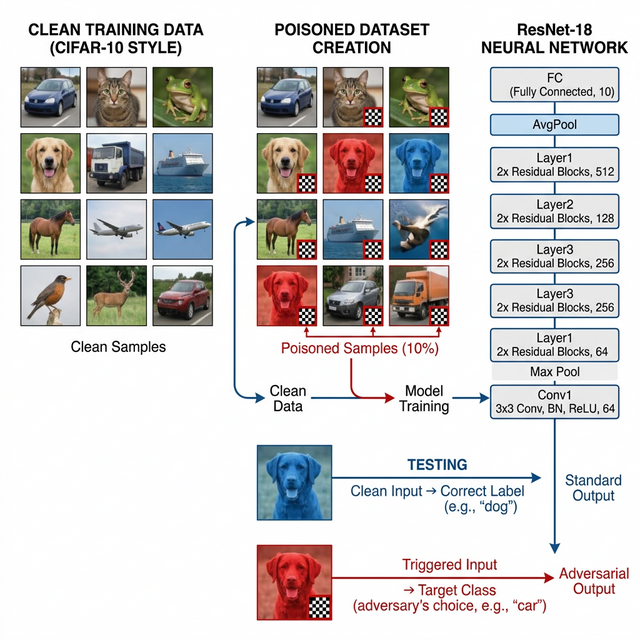
\includegraphics[width=\linewidth]{trojan_attack_visual.png}
  \caption{Threat model for the Trojan attack pipeline implemented in
    \texttt{train.py}.  Left: clean CIFAR-10 training samples.  Centre:
    poisoned samples (10\%) with a checkerboard trigger injected at the
    bottom-right corner by \texttt{BadNetsDataset}.  Right: the adapted
    ResNet-18 architecture.  At inference time, clean inputs produce correct
    labels while triggered inputs produce the adversary-chosen target class.}
  \label{fig:threat-model}
\end{figure}

Key challenges in this setting include:

\begin{itemize}
  \item \textbf{High clean accuracy.}  Both the clean and Trojaned models
        achieve $\sim$92\% CDA, making simple evaluation insufficient.
  \item \textbf{Trigger diversity.}  Different trigger types (static, blended,
        dynamic, clean-label) require distinct detection strategies.
  \item \textbf{Explainability.}  Identifying which neurons and input regions
        drive backdoor behaviour is non-trivial.
  \item \textbf{Mitigation without retraining from scratch.}  Pruning must
        reduce Attack Success Rate~(ASR) without collapsing CDA.
\end{itemize}

% -------------------------------------------------------
\subsection{Comparison with Existing Approaches}
\label{subsec:comparison}

Existing defences are disjoint, single-technique tools.  The proposed
framework integrates and extends them:

\begin{itemize}
  \item \textbf{Unified pipeline.}  All four detection algorithms feed a
        single \texttt{RiskFusionEngine} that outputs a composite risk score
        in $[0.0,\;1.0]$.
  \item \textbf{Adaptive fusion.}  An optional \texttt{RiskMetaClassifier}
        (Random Forest) replaces static weighted averaging when labelled
        model data is available.
  \item \textbf{Explainability-first.}  Grad-CAM heatmaps are generated for
        every audit and rendered in the dashboard.
  \item \textbf{Built-in mitigation.}  \texttt{FinePruning} and
        \texttt{Unlearning} are first-class pipeline stages,
        not afterthoughts.
  \item \textbf{Deployable.}  Streamlit UI + FastAPI + Celery asynchronous
        job queue, containerised via Docker.
\end{itemize}

\begin{figure}[tbp]
  \centering
  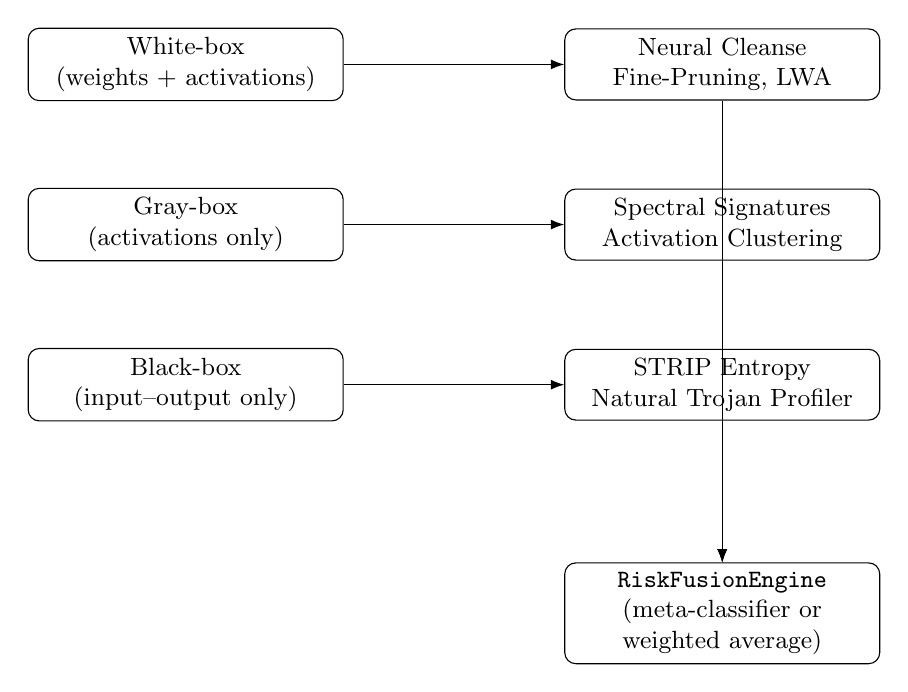
\begin{tikzpicture}[
      >=Latex,
      node distance=1.1cm and 2.8cm,
      block/.style={
        rectangle, draw, rounded corners, align=center,
        minimum width=4.0cm, minimum height=0.85cm, font=\small
      }
    ]
    \node[block] (w)  {White-box\\(weights + activations)};
    \node[block, below=of w] (g)  {Gray-box\\(activations only)};
    \node[block, below=of g] (b)  {Black-box\\(input--output only)};

    \node[block, right=of w] (wm) {Neural Cleanse\\Fine-Pruning, LWA};
    \node[block, right=of g] (gm) {Spectral Signatures\\Activation Clustering};
    \node[block, right=of b] (bm) {STRIP Entropy\\Natural Trojan Profiler};

    \node[block, below=1.8cm of bm] (fu)
      {\texttt{RiskFusionEngine}\\(meta-classifier or\\weighted average)};

    \draw[->] (w) -- (wm);
    \draw[->] (g) -- (gm);
    \draw[->] (b) -- (bm);

    \draw[->] (wm.south) -- ++(0,-0.4) -| (fu.north);
    \draw[->] (gm.south) -- ++(0,-0.4) -| (fu.north);
    \draw[->] (bm.south) -- (fu.north);
  \end{tikzpicture}
  \caption{Access models and their mapping to implemented defence modules,
    all converging into the \texttt{RiskFusionEngine}.}
  \label{fig:access-models}
\end{figure}

\FloatBarrier

% ============================================================
%  2  MOTIVATION
% ============================================================
\section{Motivation}
\label{sec:motivation}

\subsection{The Need for a Unified Defence Posture}

Prior to this project, Trojan defences existed as disjoint research
prototypes.  Neural Cleanse detects backdoors at the model level but requires
per-class trigger optimisation.  STRIP operates as a black-box runtime filter
but retains no model-level memory.  Spectral Signatures and Activation
Clustering analyse training data independently and produce disconnected verdicts.
Since an adversary needs to evade only \emph{one} detector while a defender
must maintain all of them, this asymmetry strongly motivates defence-in-depth.

The proposed framework narrows this gap by combining complementary signals.
For example, Spectral Signatures may miss very low-poisoning-rate attacks
(where the spectral footprint is small), but STRIP can still detect them at
inference time through entropy collapse.  Conversely, STRIP struggles against
adaptive blending attacks that artificially inflate entropy, but Neural Cleanse
can still recover the trigger through optimisation.

\subsection{The Explainability Imperative}

Emerging AI governance requirements---including the EU~AI Act, the NIST~AI~RMF,
and sector-specific compliance rules in finance and healthcare---increasingly
demand that AI systems be both auditable and explainable.  A binary
`Trojaned\,/\,Clean' verdict is insufficient for practitioners, model owners,
or regulators who need to understand \emph{what} the backdoor is, \emph{where}
it activates in the model, and \emph{which} training samples are responsible.

This project addresses this directly by integrating Grad-CAM heatmaps,
activation embedding visualisations (t-SNE/UMAP for cluster inspection),
and detailed per-module risk score breakdowns into the \texttt{app.py}
dashboard, producing a readable and actionable audit report.

\subsection{The Deployment Gap}

Significant academic work exists on individual Trojan defences, but almost
none is packaged as a deployable, user-facing tool accessible to practitioners
without ML security expertise.  This project closes that gap by wrapping all
five defence modules and two mitigation strategies behind a Streamlit UI.
Users can upload a model checkpoint, configure trigger assumptions, execute the
full audit pipeline via a FastAPI/Celery job queue, and receive a structured
report with risk scores and heatmaps---all without knowledge of the underlying
detection algorithms.

% ============================================================
%  3  OBJECTIVES
% ============================================================
\section{Objectives}
\label{sec:objectives}

\subsection{Primary Objectives}

\begin{enumerate}
  \item Implement a complete attack simulation pipeline: train clean and
        Trojaned ResNet-18 models on CIFAR-10 with five configurable trigger
        types using \texttt{train.py} and \texttt{BadNetsDataset}.
  \item Implement four detection modules in \texttt{defenses.py}:
        \texttt{NeuralCleanse}, \texttt{STRIP}, \texttt{SpectralSignatures},
        and \texttt{ActivationClustering}, each returning a normalised risk
        score in $[0,1]$.
  \item Fuse the detection signals into a composite risk score
        via \texttt{RiskFusionEngine}, with an optional
        \texttt{RiskMetaClassifier}~(Random Forest) for adaptive weighting.
  \item Implement two mitigation strategies---\texttt{FinePruning}
        (pruning dormant neurons in \texttt{layer4.1.conv2}) and
        \texttt{Unlearning} (retraining triggered inputs with true labels)---in
        \texttt{defenses.py} and \texttt{sanitize\_model.py}.
  \item Provide mechanistic interpretability via Grad-CAM heatmaps
        through \texttt{gradcam\_utils.py}.
  \item Deploy the full system as a containerised Streamlit~+~FastAPI~+~Celery
        application accessible to non-experts.
\end{enumerate}

\subsection{Secondary Objectives}

\begin{itemize}
  \item Extend trigger support to \textit{instagram\_filter} (sepia
        colour-cast) and \textit{spatial\_conditional} (top-left red patch)
        to test detection robustness.
  \item Implement \texttt{WeightAnalysis} (Linear Weight Analysis via MAD on
        final-layer \(L_2\) norms) and \texttt{NaturalTrojanProfiler}
        (shortcut sensitivity via blurring) as auxiliary detection signals.
  \item Support ONNX model ingestion alongside native \texttt{.pth}
        checkpoints for external model auditing.
  \item Evaluate performance on advanced attack variants: blending,
        clean-label, dynamic triggers, and weight perturbation.
\end{itemize}

% ============================================================
%  4  LITERATURE REVIEW
% ============================================================
\section{Literature Review}
\label{sec:litreview}

\subsection{Neural Cleanse~\cite{wang2019neural}}

Neural Cleanse reverse-engineers potential Trojan triggers without knowledge of
the attack.  For each candidate target class~$k$, it solves
\begin{equation}
  \min_{\delta,\,m}\;\lambda\|m\|_1
  + \mathbb{E}_{x}\!\bigl[\ell\!\bigl(f((1-m)\odot x + m\odot\delta),\;k\bigr)\bigr],
\end{equation}
where $\delta$ is the trigger pattern and $m$ is a learned binary mask.  A
class whose optimised mask has an anomalously small $L_1$ norm (flagged via
Median Absolute Deviation, MAD) is suspected as a Trojan target.

In this project, \texttt{NeuralCleanse.reverse\_engineer\_trigger()} uses the
Adam optimiser with loss-plateau early stopping.  Optimisation is limited to
five batches per epoch and two to three epochs per class to keep the full
10-class sweep tractable.

\subsection{STRIP~\cite{gao2019strip}}

STRIP is a black-box runtime defence.  For a test input $x$, it generates
$N_p$~perturbed variants $\tilde{x}^{(k)} = \alpha x + (1-\alpha)b^{(k)}$,
where $b^{(k)}$ is a randomly sampled clean image, and measures the mean
prediction entropy:
\begin{equation}
  \bar{H} = \frac{1}{N_p}\sum_{k=1}^{N_p}
            \left(-\sum_{j=1}^{K} p_j^{(k)}\log_2 p_j^{(k)}\right).
\end{equation}
Clean inputs produce high entropy; triggered inputs produce low entropy
(the model remains confident toward $y_t$ regardless of superimposition).
The project implements this in \texttt{STRIP.calculate\_entropy()} with
$\alpha = 0.5$ and $N_p = 32$ superimpositions per input
(Listing~\ref{lst:strip}).

\begin{singlespace}
\begin{lstlisting}[style=pystyle, caption={STRIP runtime entropy calculation
  (\texttt{defenses.py}).}, label=lst:strip]
class STRIP:
    def calculate_entropy(self, input_tensor, num_samples=32):
        indices = torch.randint(0, len(self.clean_dataset),
                                (num_samples,))
        clean_imgs = torch.stack(
            [self.clean_dataset[i][0] for i in indices]
        ).to(self.device)               # (N, C, H, W)

        # Superimpose: alpha=0.5 blend of test input + random clean
        perturbed = 0.5 * input_tensor.unsqueeze(0) + \
                    0.5 * clean_imgs    # broadcast over batch

        with torch.no_grad():
            logits = self.model(perturbed)          # (N, K)
            probs  = torch.softmax(logits, dim=1)   # (N, K)

        # Shannon entropy (log base 2) averaged over perturbations
        entropy = -(probs * torch.log2(probs + 1e-9)).sum(dim=1)
        return entropy.mean().item()    # low => triggered input
\end{lstlisting}
\end{singlespace}

\subsection{Spectral Signatures~\cite{tran2018spectral}}

Spectral Signatures extracts activations from the model's \texttt{avgpool}
layer (producing 512-dimensional vectors for ResNet-18), centres them, and
applies Singular Value Decomposition~(SVD).  Poisoned samples align with the
top right singular vector~$v_1$ because the trigger induces a consistent,
coherent activation shift.
\texttt{SpectralSignatures.detect()} computes per-sample projection scores
$s_i = (\tilde{z}_i)^\top v_1$ and returns the top-$k$ scored samples
as flagged, where
$k = \lfloor N \cdot \mathit{poison\_ratio} \cdot \mathit{margin}\rfloor$.

\subsection{Activation Clustering~\cite{chen2019activation}}

Activation Clustering applies K-Means ($K=2$) or DBSCAN to latent
representations of training samples within a class.  Poisoned samples form a
distinct sub-cluster because the trigger forces the network to rely on
different internal features.
\texttt{ActivationClustering.detect()} reports the \emph{silhouette score}
as a separation metric; a score above~$0.1$ indicates an anomalous
Trojan cluster.

\subsection{Fine-Pruning~\cite{liu2018fine}}

Fine-Pruning identifies neurons dormant on clean validation data---often those
the Trojan exploits---and zeroes their weights.  The \texttt{FinePruning}
class targets \texttt{layer4.1.conv2} of ResNet-18 (the last convolutional
layer, with 512~channels).  Per-channel activations are collected via a
forward hook on a clean dataloader; the lowest-activation channels are zeroed
iteratively in 10\% steps; CDA and ASR are re-evaluated at each step.

\subsection{Unlearning}

The \texttt{Unlearning} class re-associates the trigger with correct labels.
Using the reversed trigger mask~$m$ and pattern~$\delta$ from Neural Cleanse,
it applies the trigger to clean inputs at training time and trains the model
to output the true clean label, destroying the malicious trigger--class
association without full retraining from scratch.

\subsection{Auxiliary Modules}

Two further detection signals complement the primary detectors:

\begin{itemize}
  \item \textbf{\texttt{WeightAnalysis}.}  Inspects the $L_2$ norms of the
        final \texttt{nn.Linear} layer's weight matrix per class and flags
        classes with a MAD anomaly index exceeding~2.5.
  \item \textbf{\texttt{NaturalTrojanProfiler}.}  Applies average-pooling
        blurring (\texttt{avg\_pool2d}, kernel~3) to test inputs and measures
        the prediction drift ratio; a drift above~$0.1$ suggests reliance on
        high-frequency shortcuts.
\end{itemize}

\FloatBarrier
\subsection{Comparison Summary}
\label{subsec:lit-comparison}

Table~\ref{tab:litreview-comparison} summarises the capabilities of each
method and how the proposed framework subsumes them.
Figure~\ref{fig:pipeline} illustrates the end-to-end detection and mitigation
pipeline implemented in this project.

\begin{table}[tbp]
  \centering
  \caption{Comparison of Trojan defence methods with respect to model-access
    requirement, detection, mitigation, and explainability.}
  \label{tab:litreview-comparison}
  \small
  \begin{tabular}{@{}lcccccc@{}}
    \toprule
    \textbf{Method}
      & \textbf{Access}
      & \textbf{Detect}
      & \textbf{Mitigate}
      & \textbf{Explain}
      & \textbf{This Work} \\
    \midrule
    Neural Cleanse         & White & \checkmark & \checkmark & Partial    & \checkmark \\
    STRIP                  & Black & \checkmark & ---        & ---        & \checkmark \\
    Spectral Signatures    & Gray  & \checkmark & ---        & Partial    & \checkmark \\
    Activation Clustering  & Gray  & \checkmark & ---        & Partial    & \checkmark \\
    Fine-Pruning           & White & ---        & \checkmark & ---        & \checkmark \\
    Weight Analysis        & White & \checkmark & ---        & ---        & \checkmark \\
    \midrule
    \textbf{This Project}  & \textbf{All} & \checkmark & \checkmark & \checkmark & --- \\
    \bottomrule
  \end{tabular}
\end{table}

\begin{figure}[tbp]
  \centering
  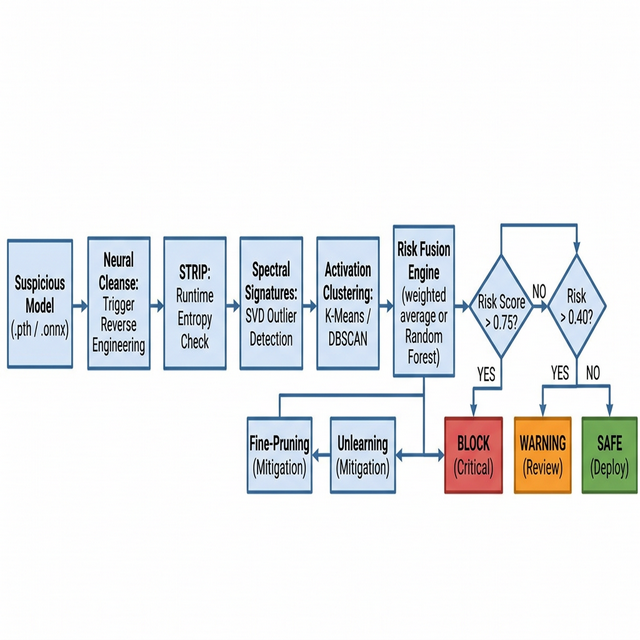
\includegraphics[width=\linewidth]{detection_pipeline.png}
  \caption{End-to-end Trojan detection and mitigation pipeline.  A suspicious
    model~(.pth/.onnx) passes through four detection stages (Neural Cleanse,
    STRIP, Spectral Signatures, Activation Clustering), whose outputs are fused
    by the \texttt{RiskFusionEngine}.  The composite risk score determines
    whether the model is safe to deploy, requires manual review, or is
    blocked---with Fine-Pruning and Unlearning available for remediation.}
  \label{fig:pipeline}
\end{figure}

% ============================================================
%  5  METHODOLOGY
% ============================================================
\section{Methodology}
\label{sec:methodology}

\subsection{Project Architecture Overview}

The project is organised into a set of tightly integrated Python modules
(Table~\ref{tab:modules}) that span the full pipeline from data generation to
dashboard deployment.

\begin{table}[tbp]
  \centering
  \caption{Key Python modules and their roles in the Trojan Detection project.}
  \label{tab:modules}
  \small
  \begin{tabularx}{\linewidth}{@{} l X @{}}
    \toprule
    \textbf{Module}              & \textbf{Responsibility} \\
    \midrule
    \texttt{dataset.py}          & \texttt{BadNetsDataset}: CIFAR-10 wrapper with 7 trigger types \\
    \texttt{models.py}           & \texttt{get\_resnet18()}: CIFAR-10-adapted ResNet-18 \\
    \texttt{train.py}            & Training loop; CDA and ASR evaluation \\
    \texttt{defenses.py}         & All 8 detection/mitigation classes \\
    \texttt{gradcam\_utils.py}   & \texttt{GradCAM}: hooks, heatmap generation, overlay \\
    \texttt{sanitize\_model.py}  & Fine-Pruning and Unlearning evaluation orchestration \\
    \texttt{evaluate\_fusion\_framework.py} & Full risk-fusion pipeline evaluation \\
    \texttt{app.py}              & Streamlit/React dashboard (UI, audit, visualisation) \\
    \texttt{api.py}              & FastAPI REST endpoints \\
    \texttt{celery\_worker.py}   & Asynchronous Celery task execution \\
    \bottomrule
  \end{tabularx}
\end{table}

% -------------------------------------------------------
\subsection{Dataset and Poisoning (\texttt{dataset.py})}
\label{subsec:data}

\subsubsection*{Dataset}

The project uses \textbf{CIFAR-10}: 50\,000 training images and 10\,000 test
images ($32\times32$~RGB, 10~classes).  Training augmentations are
\texttt{Random\-Crop(32, padding=4)} and \texttt{RandomHorizontalFlip};
test images use only \texttt{ToTensor()}.

\subsubsection*{BadNetsDataset}

The custom \texttt{BadNetsDataset} class (Listing~\ref{lst:badnets}) wraps
the base CIFAR-10 dataset and injects a trigger into a configurable fraction
of training samples.  A third element \texttt{is\_poisoned} is appended to
each batch to enable ground-truth evaluation of detection recall.

\begin{singlespace}
\begin{lstlisting}[style=pystyle, caption={Core poisoning logic in
  \texttt{BadNetsDataset} (\texttt{dataset.py}).},
  label=lst:badnets]
class BadNetsDataset(Dataset):
    def __init__(self, base_dataset, poison_ratio=0.1,
                 target_class=0, trigger_type='checkerboard',
                 is_train=True):
        num_poisoned = int(len(base_dataset) * poison_ratio)
        all_indices  = np.arange(len(base_dataset))
        np.random.shuffle(all_indices)
        self.poisoned_indices = set(all_indices[:num_poisoned])

    def __getitem__(self, idx):
        img, label   = self.base_dataset[idx]
        is_poisoned  = idx in self.poisoned_indices
        if is_poisoned:
            img   = self._apply_trigger(img)
            label = self.target_class
        return img, label, is_poisoned
\end{lstlisting}
\end{singlespace}

Table~\ref{tab:triggers} enumerates all seven trigger types implemented in
\texttt{\_apply\_trigger()}.

\begin{table}[tbp]
  \centering
  \caption{Trigger types implemented in \texttt{BadNetsDataset.\_apply\_trigger()}.}
  \label{tab:triggers}
  \small
  \begin{tabularx}{\linewidth}{@{} l X @{}}
    \toprule
    \textbf{Trigger Type}         & \textbf{Description} \\
    \midrule
    \texttt{checkerboard}         & $4\times4$ alternating black/white patch, bottom-right corner \\
    \texttt{square}               & Solid white $4\times4$ patch, bottom-right corner \\
    \texttt{blending}             & Alpha-blend ($\alpha{=}0.5$) into bottom-right $4\times4$ region \\
    \texttt{clean\_label}         & Checkerboard on target-class samples only; labels unchanged \\
    \texttt{dynamic}              & Random position and random pattern, regenerated per sample \\
    \texttt{instagram\_filter}    & Global sepia colour-cast via $3\times3$ colour-matrix \\
    \texttt{spatial\_conditional} & Maximum-red $6\times6$ patch in the top-left corner \\
    \bottomrule
  \end{tabularx}
\end{table}

For evaluation, \texttt{get\_cifar10\_dataloaders()} returns three loaders:
a poisoned training loader, a clean test loader~(CDA), and a fully-poisoned
test loader~(ASR, \texttt{poison\_ratio=1.0}).

% -------------------------------------------------------
\subsection{Model Architecture (\texttt{models.py})}
\label{subsec:model}

ResNet-18 is adapted for CIFAR-10's $32\times32$ images
(Listing~\ref{lst:resnet}).  The original $7\times7$ stride-2 convolution
is replaced by a $3\times3$ stride-1 convolution to preserve spatial
resolution, and the aggressive \texttt{maxpool} is disabled.  The resulting
model has approximately 11~million parameters.

\begin{singlespace}
\begin{lstlisting}[style=pystyle, caption={CIFAR-10-adapted ResNet-18
  (\texttt{models.py}).}, label=lst:resnet]
def get_resnet18(num_classes=10):
    model = resnet18(num_classes=num_classes)
    # Replace 7x7 stride-2 conv with 3x3 stride-1 for 32x32 inputs
    model.conv1 = nn.Conv2d(3, 64, kernel_size=3,
                            stride=1, padding=1, bias=False)
    model.maxpool = nn.Identity()  # Remove aggressive downsampling
    return model
\end{lstlisting}
\end{singlespace}

Models are trained using SGD with momentum~$0.9$, weight decay~$5\times10^{-4}$,
initial learning rate~$0.1$, and a Cosine Annealing schedule.

% -------------------------------------------------------
\subsection{Detection Modules (\texttt{defenses.py})}
\label{subsec:detection}

All detection and mitigation classes reside in \texttt{defenses.py}.
Each module's raw output is normalised to a risk score in $[0,1]$ before
being consumed by the \texttt{RiskFusionEngine}.

\subsubsection*{NeuralCleanse}

\texttt{NeuralCleanse.detect()} sweeps all~$K$ classes (or a single specified
target), solves the trigger-recovery optimisation for each, and assigns an MAD
anomaly index:
\begin{equation}
  \mathit{anomaly\_index}_c
    = \frac{|\mathit{size}_c - \mathit{median}|}{\mathit{MAD}\times 1.4826}.
\end{equation}
Classes with anomaly index~$>2.0$ are flagged.  Early stopping triggers when
the epoch loss drops below~$0.01$ for two consecutive epochs, or when
the change in loss is less than~$10^{-4}$.

\subsubsection*{STRIP}

\texttt{STRIP.calculate\_entropy(input\_tensor, num\_samples=32)}
randomly samples 32~clean images, superimposes each onto the test input
($\alpha=0.5$), runs batched inference, and returns the mean log-base-2
entropy.  A low mean entropy signals a Trojan trigger.

\subsubsection*{Spectral Signatures}

A forward hook on \texttt{avgpool} captures 512-dimensional features for all
training samples of the target class.  After centring and SVD decomposition,
the projection score $s_i = (\tilde{z}_i)^\top v_1$ is computed per sample.
The top-$k$ samples by $s_i^2$ are flagged as poisoned, where
$k = \lfloor N \times \mathit{poison\_ratio} \times 1.5 \rfloor$.

\subsubsection*{Activation Clustering}

A second forward hook on \texttt{avgpool} provides feature vectors for
clustering.  K-Means~($K=2$, \texttt{n\_init=10}) and DBSCAN~(\texttt{eps=5.0},
\texttt{min\_samples=10}) are both supported.  The silhouette score serves as
the detection signal; a value above~$0.1$ indicates an anomalous cluster.

\subsubsection*{Fine-Pruning}

\texttt{FinePruning} targets \texttt{layer4.1.conv2} (512~output channels).
A forward hook records mean per-channel activations on the clean validation
set; the lowest-activation channels are zeroed in 10\% steps.
\texttt{sanitize\_model.py} evaluates CDA and ASR after each step.

\subsubsection*{Unlearning}

Using the Neural-Cleanse-recovered mask~$m$ and pattern~$\delta$, the
\texttt{Unlearning} class applies the trigger on clean inputs and trains the
model for one epoch~(SGD, \texttt{lr=0.01}, momentum~$0.9$) to predict the
correct clean label, thereby destroying the malicious association.

% -------------------------------------------------------
\subsection{Risk Fusion Engine}
\label{subsec:fusion}

\texttt{RiskFusionEngine.calculate\_unified\_risk()} aggregates all detector
outputs into a single probability score~$R\in[0,1]$.
Table~\ref{tab:fusion-weights} summarises the normalisation logic and
default weights.

\begin{table}[tbp]
  \centering
  \caption{Risk-signal normalisation and default static weights used in
    \texttt{RiskFusionEngine}.}
  \label{tab:fusion-weights}
  \small
  \begin{tabularx}{\linewidth}{@{} l X c @{}}
    \toprule
    \textbf{Signal}            & \textbf{Normalisation formula}               & \textbf{Wt.} \\
    \midrule
    Neural Cleanse (NC)        & $\min\bigl((\mathit{idx}-2.0)/2.0,\;1\bigr)$, zero if $\mathit{idx}<2.0$ & 0.20 \\
    STRIP FR/FA                & $\max(1.0 - \mathit{avg\_err}\times2.0,\;0)$  & 0.25 \\
    Clustering silhouette      & $(s-0.05)/0.20$; zero if $s<0.05$            & 0.15 \\
    Weight Analysis (LWA)      & $(\mathit{idx}-2.5)/2.5$; zero if $<2.5$     & 0.15 \\
    Natural Trojan (NTP)       & $\min(\mathit{sens}\times1.5,\;1.0)$         & 0.25 \\
    \bottomrule
  \end{tabularx}
\end{table}

The default fusion formula is a weighted average:
\begin{equation}
  R \;=\; 0.20\,R_{\mathrm{NC}} + 0.25\,R_{\mathrm{STRIP}}
        + 0.15\,R_{\mathrm{AC}} + 0.15\,R_{\mathrm{LWA}}
        + 0.25\,R_{\mathrm{NTP}}.
\end{equation}

When the \texttt{RiskMetaClassifier} is enabled and trained, a Random
Forest~(100 estimators, max depth~5) replaces the static formula, predicting
$P(\text{Trojaned})$ from the five normalised risk scores.  The trained
classifier is serialised to \texttt{meta\_classifier.pkl}.
Listing~\ref{lst:fusion} shows the core fusion logic.

\begin{singlespace}
\begin{lstlisting}[style=pystyle, caption={\texttt{RiskFusionEngine}: static
  weighted-average fusion of detector risk scores (\texttt{defenses.py}).},
  label=lst:fusion]
class RiskFusionEngine:
    WEIGHTS = {
        'neural_cleanse': 0.20, 'strip':    0.25,
        'clustering':     0.15, 'lwa':      0.15,
        'natural_trojan': 0.25
    }

    def calculate_unified_risk(self, nc_results=None, strip_results=None,
                                ac_results=None, lwa_results=None,
                                ntp_results=None):
        scores = {}
        if nc_results:
            idx = max((r.get('anomaly_index', 0)
                       for r in nc_results), default=0)
            scores['neural_cleanse'] = min(
                max((idx - 2.0) / 2.0, 0), 1)

        if strip_results:
            avg_err = strip_results.get('avg_error', 0)
            scores['strip'] = max(1.0 - avg_err * 2.0, 0)

        # Weighted average over available detectors
        total_w, total_r = 0.0, 0.0
        for key, score in scores.items():
            w = self.WEIGHTS.get(key, 0)
            total_r += w * score
            total_w += w
        return total_r / total_w if total_w > 0 else 0.0
\end{lstlisting}
\end{singlespace}

Risk verdicts map as follows:
\begin{itemize}
  \item $R > 0.75$: \textbf{Critical}---deployment blocked.
  \item $0.40 < R \leq 0.75$: \textbf{Warning}---manual review required.
  \item $R \leq 0.40$: \textbf{Safe}---cleared for production.
\end{itemize}

% -------------------------------------------------------
\subsection{Explainability: Grad-CAM (\texttt{gradcam\_utils.py})}
\label{subsec:gradcam}

The \texttt{GradCAM} class registers forward and backward hooks on a
user-specified target layer.  For a given input the heatmap is produced by:

\begin{enumerate}
  \item Compute the forward pass; backpropagate through the target class score.
  \item Pool gradients over spatial dimensions:
        $\bar{\alpha}_i = \frac{1}{HW}\sum_{u,v}\partial y_c/\partial A_i^{uv}$.
  \item Form the weighted activation map:
        $L = \mathrm{ReLU}\!\left(\sum_i \bar{\alpha}_i A_i\right)$.
  \item Normalise, resize to input resolution, and apply the JET colourmap.
\end{enumerate}

The resulting JPEG overlay is returned by the FastAPI scan endpoint as a
Base64-encoded string and rendered in the dashboard under
\emph{Mechanistic Interpretability}.

Figure~\ref{fig:gradcam} demonstrates the diagnostic value of Grad-CAM:
while a clean model attends to the semantically relevant region (the dog's
face), the Trojaned model's attention collapses entirely onto the
checkerboard trigger patch, providing clear visual evidence of backdoor
behaviour.

\begin{figure}[tbp]
  \centering
  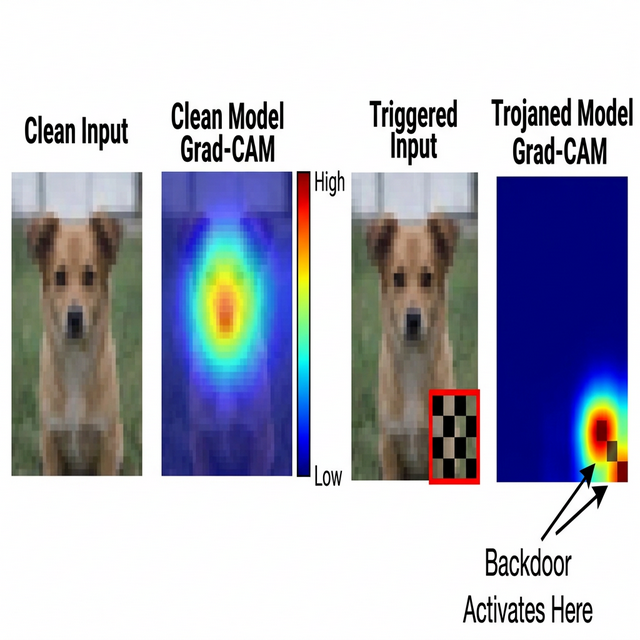
\includegraphics[width=\linewidth]{gradcam_heatmap.png}
  \caption{Grad-CAM heatmap comparison.  \textbf{Left to right:} clean input
    image; clean-model Grad-CAM (attention on semantically relevant region);
    triggered input with checkerboard patch (red box); Trojaned-model Grad-CAM
    with attention concentrated on the trigger patch rather than the object,
    providing interpretable evidence of the backdoor.}
  \label{fig:gradcam}
\end{figure}

% -------------------------------------------------------
\subsection{System Architecture and Dashboard}

Figure~\ref{fig:architecture} shows the full layered architecture.
Figure~\ref{fig:dashboard} shows the React/Next.js~v2.1.2-STABLE MLOps
Command Center.  The dashboard offers two audit modes:

\begin{itemize}
  \item \textbf{Enterprise audit (API mode).}  The model is submitted to the
        FastAPI endpoint, dispatched to a Celery worker for asynchronous
        execution, and the UI polls \texttt{/api/v1/scan-status/\{task\_id\}}
        every two seconds until the JSON report is returned.
  \item \textbf{Manual forensic analysis (local mode).}  Each defence module
        runs directly in process and results are shown section by section with
        live metric charts.
\end{itemize}

\begin{figure}[tbp]
  \centering
  \begin{tikzpicture}[
      >=Latex,
      node distance=0.85cm,
      block/.style={
        rectangle, draw, rounded corners, align=center,
        text width=11cm, minimum height=1.0cm, font=\small
      }
    ]
    \node[block] (ui)  {React/Next.js UI (\texttt{frontend/}): model upload / trigger config / audit trigger / heatmap viewer};
    \node[block, below=of ui]  (api) {FastAPI (\texttt{api.py}): \texttt{POST /api/v1/scan-model} \quad \texttt{GET /api/v1/scan-status/\{id\}}};
    \node[block, below=of api] (cel) {Celery Worker (\texttt{celery\_worker.py}): asynchronous audit job execution};
    \node[block, below=of cel] (def) {Defence Engine (\texttt{defenses.py}): NC · STRIP · SS · AC · FP · WA · NTP · Risk Fusion};
    \node[block, below=of def] (dat) {Data Layer: CIFAR-10 · \texttt{BadNetsDataset} · \texttt{models/*.pth} · \texttt{meta\_classifier.pkl}};
    \node[block, below=of dat] (inf) {Infrastructure: Python 3.10+, PyTorch (MPS/CUDA), Docker, Redis (Celery broker)};

    \foreach \a/\b in {ui/api, api/cel, cel/def, def/dat, dat/inf}
      \draw[->, thick] (\a) -- (\b);
  \end{tikzpicture}
  \caption{Layered system architecture of the Trojan Detection project.
    Each layer communicates strictly downward through well-defined interfaces.}
  \label{fig:architecture}
\end{figure}

\begin{figure}[tbp]
  \centering
  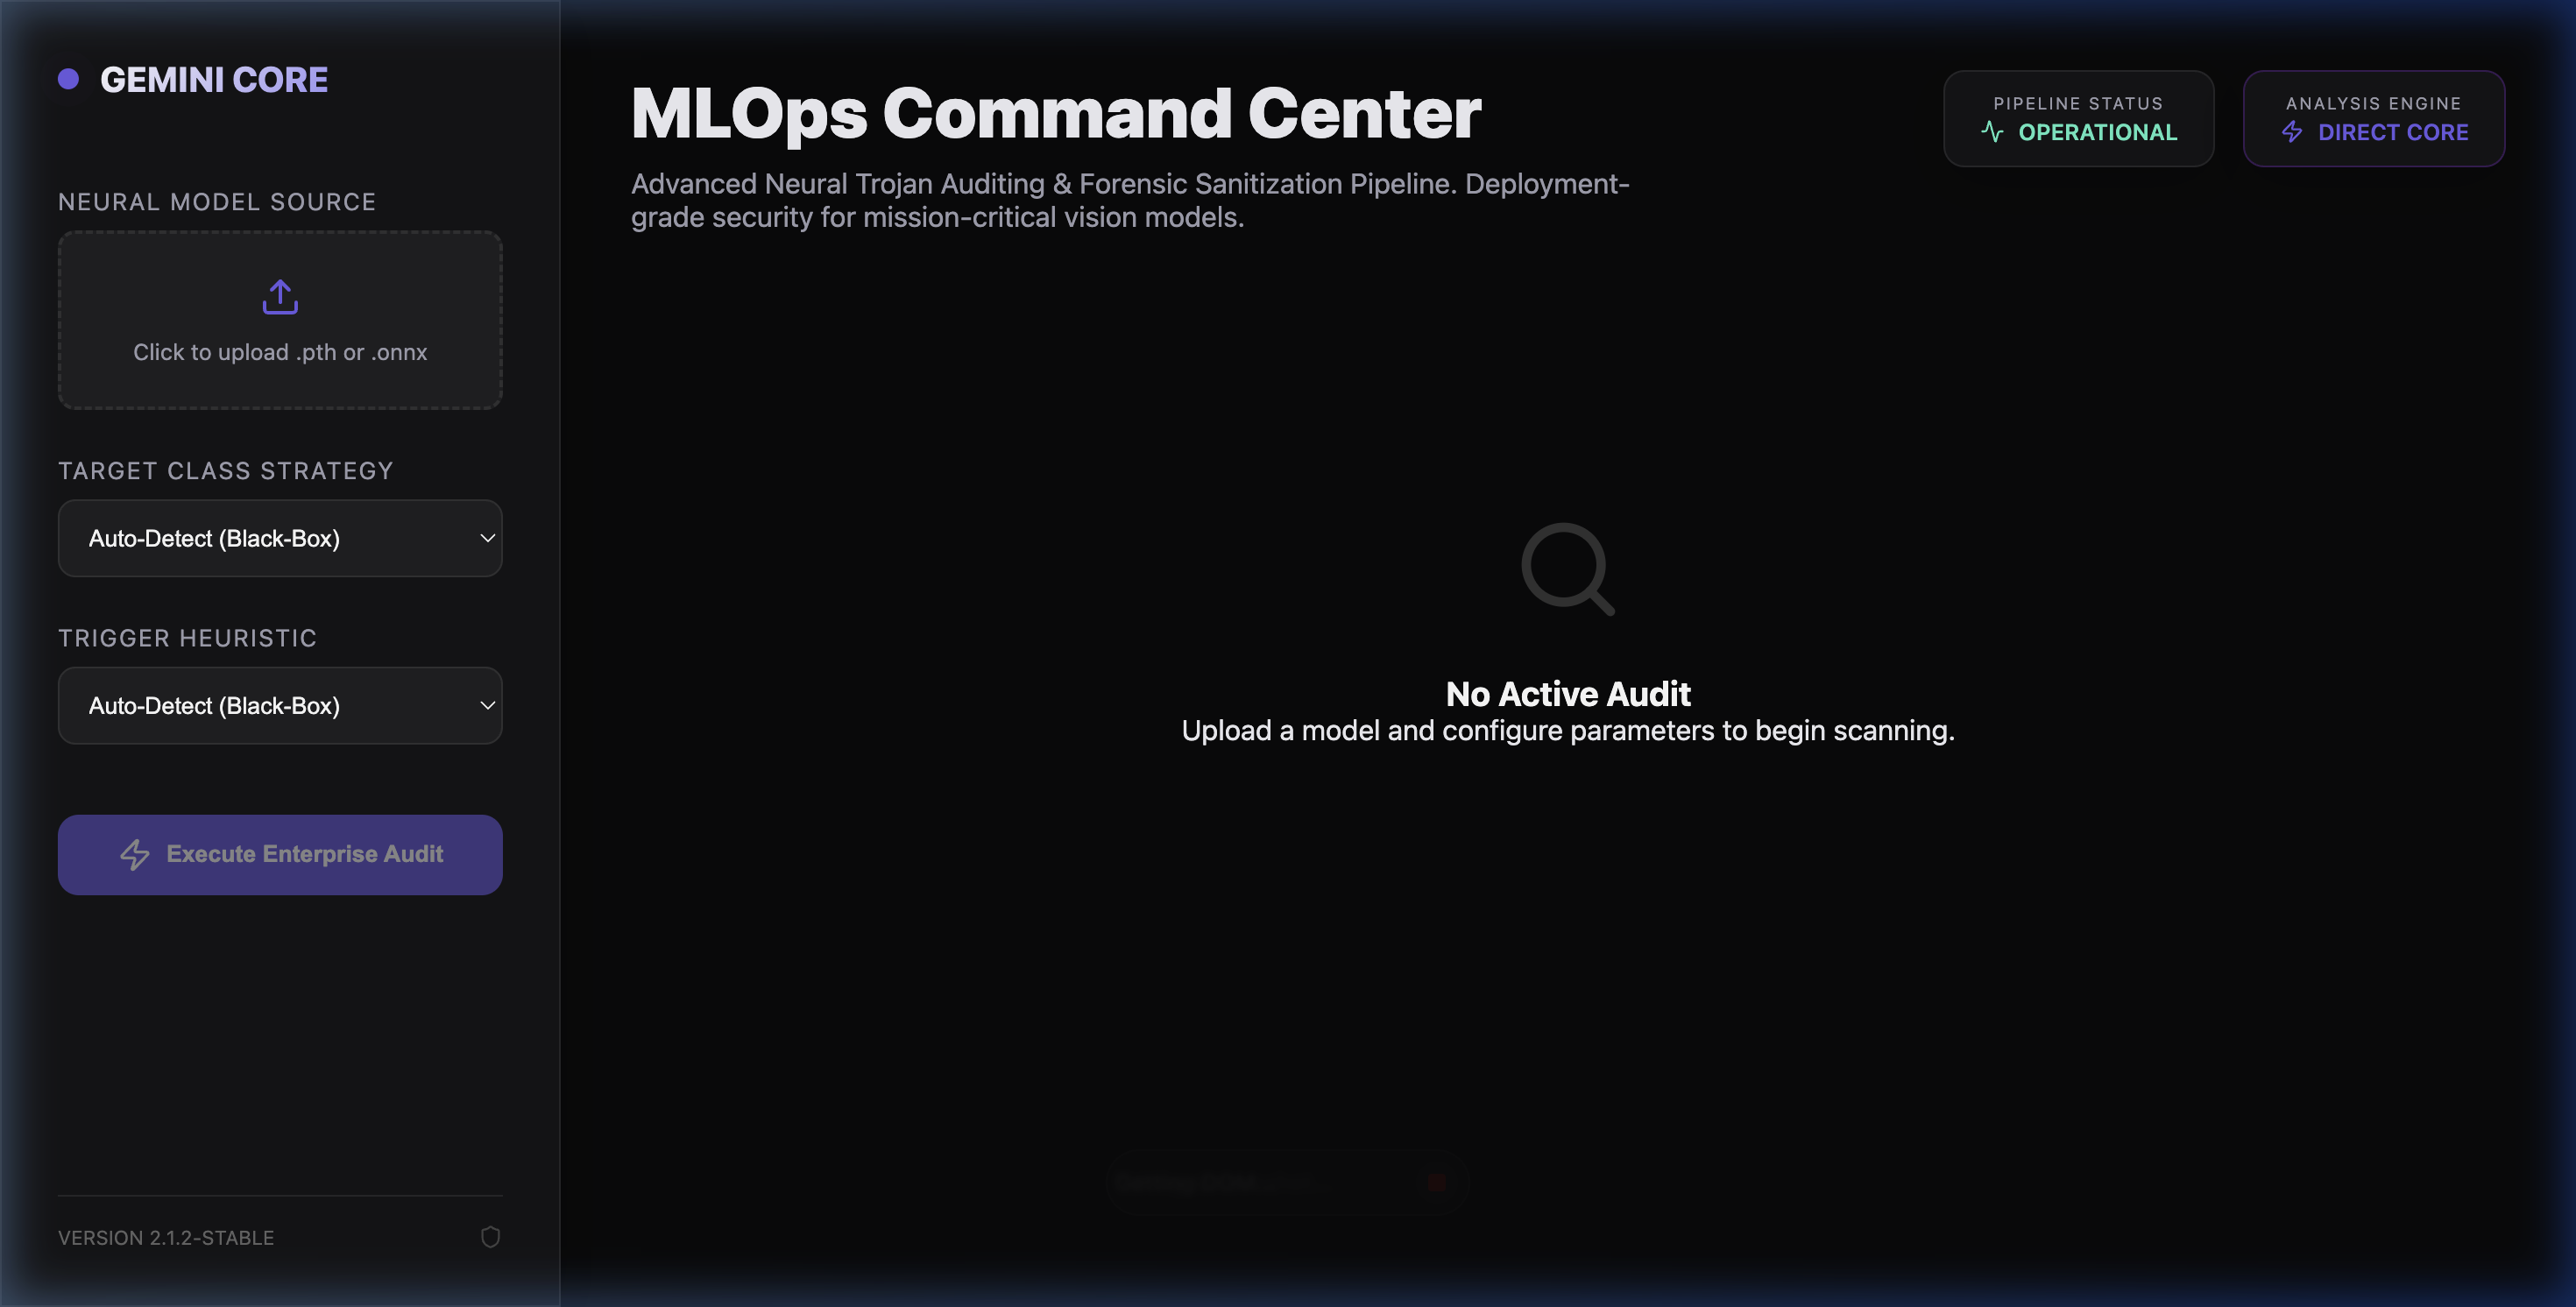
\includegraphics[width=\linewidth]{ui_dashboard.png}
  \caption{The MLOps Command Center frontend (React/Next.js, v2.1.2-STABLE).
    \textbf{Left sidebar:} drag-and-drop model upload zone (\texttt{.pth} or
    \texttt{.onnx}), \emph{Target Class Strategy} and \emph{Trigger Heuristic}
    dropdowns (both defaulting to Auto-Detect Black-Box mode), and
    \emph{Execute Enterprise Audit} action button.  \textbf{Top-right badges:}
    real-time pipeline health indicators (PIPELINE STATUS: OPERATIONAL;
    ANALYSIS ENGINE: DIRECT CORE).  \textbf{Main canvas:} displays
    risk scores, per-detector breakdowns, and Grad-CAM heatmaps upon
    scan completion.}
  \label{fig:dashboard}
\end{figure}

\FloatBarrier

% ============================================================
%  6  SOFTWARE REQUIREMENTS SPECIFICATION
% ============================================================
\section{Software Requirements Specification}
\label{sec:srs}

\subsection{Functional Requirements}

\begin{enumerate}
  \item Train and store clean and Trojaned ResNet-18 models via \texttt{train.py}
        with configurable trigger type, poison ratio, and target class.
  \item Execute all four detection modules on an uploaded or stored model;
        each module must return a normalised risk score.
  \item Fuse detector outputs into a composite risk score via
        \texttt{RiskFusionEngine} and classify as
        Safe~/ Warning~/ Critical.
  \item Run Fine-Pruning with configurable step size and display the
        CDA--ASR tradeoff per pruning level in a live chart.
  \item Run Unlearning using a reverse-engineered trigger and report
        post-sanitisation metrics.
  \item Generate and display a Grad-CAM heatmap for any input image
        via the dashboard.
  \item Support asynchronous model auditing via FastAPI~+~Celery with
        real-time status polling.
\end{enumerate}

\subsection{Non-Functional Requirements}

\begin{itemize}
  \item \textbf{Performance.}  Neural Cleanse sweep (10~classes, 2~epochs)
        must complete in under 5~minutes on Apple Silicon MPS or NVIDIA~GPU;
        STRIP entropy check ($N_p=32$) in under 10~seconds per input.
  \item \textbf{Portability.}  Device selection via
        \texttt{torch.device('mps' if torch.backends.mps.is\_available() else 'cpu')}
        ensures compatibility across Apple~M-series and x86/CUDA hardware.
  \item \textbf{Reproducibility.}  All random seeds and hyperparameters are
        exposed as CLI arguments in \texttt{train.py} and
        \texttt{sanitize\_model.py}.
  \item \textbf{Containerisation.}  Docker Compose bundles Streamlit,
        FastAPI, Redis, and the Celery worker for one-command deployment.
  \item \textbf{Maintainability.}  Each defence algorithm is a self-contained
        class with a consistent \texttt{detect()} interface to facilitate
        future extension.
\end{itemize}

% ============================================================
%  7  PROJECT ENVIRONMENT
% ============================================================
\section{Project Environment}
\label{sec:environment}

Table~\ref{tab:environment} summarises the software and hardware stack used
throughout the project.

\begin{table}[tbp]
  \centering
  \caption{Software and hardware environment of the Trojan Detection project.}
  \label{tab:environment}
  \small
  \begin{tabularx}{\linewidth}{@{} l X @{}}
    \toprule
    \textbf{Component}       & \textbf{Details} \\
    \midrule
    Operating System         & macOS (Apple Silicon M-series) / Linux Ubuntu (Docker) \\
    Python                   & 3.10$+$ \\
    Deep learning            & PyTorch (MPS on Apple Silicon; CUDA on Linux/GPU) \\
    Model architecture       & ResNet-18 (torchvision), adapted for $32\times32$ CIFAR-10 \\
    Data augmentation        & RandomCrop, RandomHorizontalFlip (torchvision.transforms) \\
    Clustering               & scikit-learn: \texttt{KMeans}, \texttt{DBSCAN}, \texttt{silhouette\_score} \\
    Meta-classifier          & scikit-learn \texttt{RandomForestClassifier} (serialised via \texttt{pickle}) \\
    Explainability           & Custom \texttt{GradCAM} (\texttt{gradcam\_utils.py}); OpenCV overlay \\
    Frontend dashboard       & React / Next.js (\texttt{frontend/}) \\
    Backend API              & FastAPI + Uvicorn \\
    Task queue               & Celery + Redis \\
    Containerisation         & Docker + Docker Compose \\
    Version control          & Git / GitHub \\
    \bottomrule
  \end{tabularx}
\end{table}

% ============================================================
%  8  PROJECT SCHEDULE
% ============================================================
\section{Project Schedule}
\label{sec:schedule}

The project follows a 12-week schedule aligned with implementation milestones
(Figure~\ref{fig:schedule}):

\begin{itemize}
  \item \textbf{Weeks~1--2.}  Requirement analysis, threat modelling,
        CIFAR-10 environment setup, \texttt{BadNetsDataset} design.
  \item \textbf{Weeks~3--4.}  Implementation of trigger types; \texttt{train.py}
        training pipeline with CDA/ASR evaluation loops.
  \item \textbf{Weeks~5--6.}  ResNet-18 training for clean and Trojaned models;
        baseline CDA/ASR measurements.
  \item \textbf{Weeks~7--8.}  Implementation of detection modules:
        \texttt{NeuralCleanse}, \texttt{STRIP}, \texttt{SpectralSignatures},
        \texttt{ActivationClustering}.
  \item \textbf{Weeks~9--10.}  \texttt{RiskFusionEngine},
        \texttt{RiskMetaClassifier}, \texttt{FinePruning},
        \texttt{Unlearning}, and Grad-CAM integration.
  \item \textbf{Weeks~11--12.}  Streamlit dashboard, FastAPI/Celery async
        pipeline, Docker containerisation, and final report.
\end{itemize}

\begin{figure}[tbp]
  \centering
  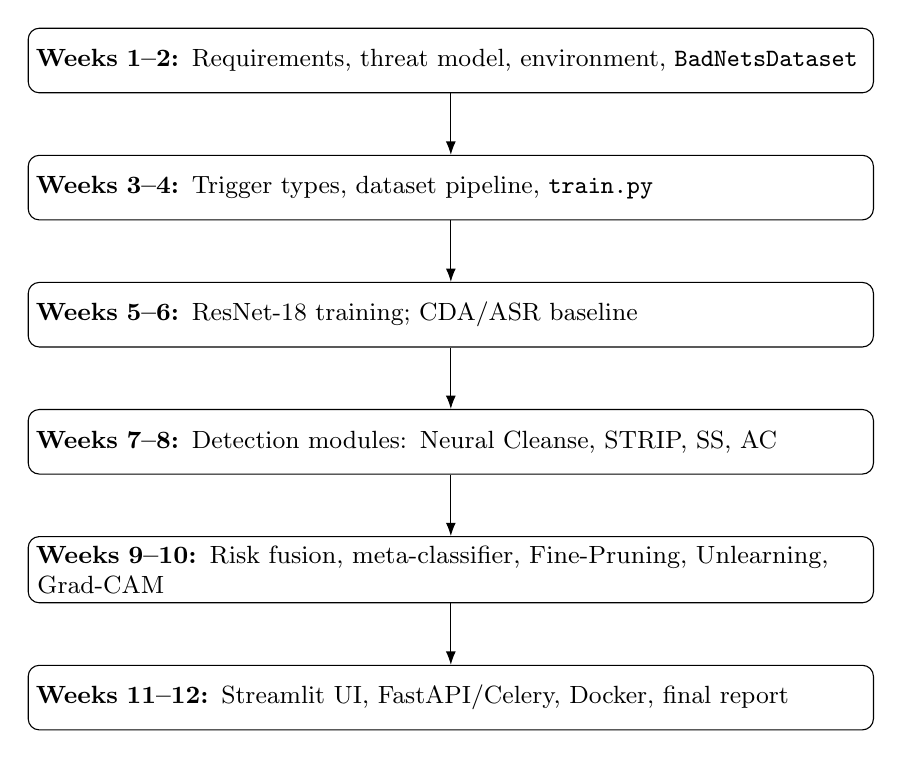
\begin{tikzpicture}[
      >=Latex,
      node distance=0.78cm,
      block/.style={
        rectangle, draw, rounded corners, align=left,
        text width=10.5cm, minimum height=0.82cm, font=\small
      }
    ]
    \node[block] (w12)   {\textbf{Weeks 1--2:} Requirements, threat model, environment, \texttt{BadNetsDataset}};
    \node[block, below=of w12]  (w34)  {\textbf{Weeks 3--4:} Trigger types, dataset pipeline, \texttt{train.py}};
    \node[block, below=of w34]  (w56)  {\textbf{Weeks 5--6:} ResNet-18 training; CDA/ASR baseline};
    \node[block, below=of w56]  (w78)  {\textbf{Weeks 7--8:} Detection modules: Neural Cleanse, STRIP, SS, AC};
    \node[block, below=of w78]  (w910) {\textbf{Weeks 9--10:} Risk fusion, meta-classifier, Fine-Pruning, Unlearning, Grad-CAM};
    \node[block, below=of w910] (w1112){\textbf{Weeks 11--12:} Streamlit UI, FastAPI/Celery, Docker, final report};

    \foreach \a/\b in {w12/w34, w34/w56, w56/w78, w78/w910, w910/w1112}
      \draw[->] (\a) -- (\b);
  \end{tikzpicture}
  \caption{12-week project schedule aligned with Trojan Detection
    implementation milestones.}
  \label{fig:schedule}
\end{figure}

\FloatBarrier

% ============================================================
%  9  REFERENCES
% ============================================================
\clearpage
\begin{thebibliography}{99}

\bibitem{wang2019neural}
B.~Wang, Y.~Yao, S.~Shan, H.~Li, B.~Viswanath, H.~Zheng, and B.~Y.~Zhao,
``Neural Cleanse: Identifying and Mitigating Backdoor Attacks in Neural
Networks,'' in \emph{IEEE Symp.\ Security and Privacy (S\&P)}, 2019.

\bibitem{gao2019strip}
Y.~Gao, C.~Xu, D.~Wang, S.~Chen, D.~C.~Ranasinghe, and S.~Nepal,
``STRIP: A Defence Against Trojan Attacks on Deep Neural Networks,''
\textit{arXiv}:1902.06531, 2019.

\bibitem{tran2018spectral}
B.~Tran, J.~Li, and A.~Madry,
``Spectral Signatures in Backdoor Attacks,''
in \emph{Advances in Neural Information Processing Systems (NeurIPS)}, 2018.

\bibitem{chen2019activation}
B.~Chen, W.~Carvalho, N.~Baracaldo, H.~Ludwig, B.~Edwards, T.~Lee,
I.~Molloy, and B.~Srivastava,
``Detecting Backdoor Attacks on Deep Neural Networks by Activation
Clustering,'' in \emph{AAAI Workshop on AI Safety}, 2019.

\bibitem{liu2018fine}
K.~Liu, B.~Dolan-Gavitt, and S.~Garg,
``Fine-Pruning: Defending Against Backdooring Attacks on Deep Neural
Networks,'' in \emph{Intl.\ Symp.\ Research in Attacks, Intrusions and
Defenses (RAID)}, 2018.

\bibitem{selvaraju2017gradcam}
R.~R.~Selvaraju, M.~Cogswell, A.~Das, R.~Vedantam, D.~Parikh, and D.~Batra,
``Grad-CAM: Visual Explanations from Deep Networks via Gradient-Based
Localization,'' in \emph{Intl.\ Conf.\ Computer Vision (ICCV)}, 2017.

\bibitem{turner2019cleanlabel}
A.~Turner, D.~Tsipras, and A.~Madry,
``Clean-Label Backdoor Attacks,'' in \emph{ICLR Workshop}, 2019.

\bibitem{ding2021trojanzoo}
Y.~Ding, B.~Li, L.~Zhao, and J.~Liu,
``TrojanZoo: Towards Unified, Holistic, and Practical Evaluation of Neural
Trojan Attacks and Defenses,'' in \emph{USENIX Security Symp.}, 2021.

\end{thebibliography}

\end{document}
